\section{Additional Visualization Examples}\label{appendix:add}

We present additional visualization examples drawn from the DA-Code, and MatplotBench to illustrate \methodname{}'s performance. For each example, we show the natural language query, the ground truth visualization, and the output generated by \methodname{}. These instances highlight \methodname{}'s ability to handle complex data patterns, ambiguous queries, and multi-file inputs through collaborative agentic refinement, often producing outputs that closely match or exceed ground truth fidelity.

\subsection{DA-Code Example}
\subsubsection{Example 1}
\begin{minted}[fontsize=\footnotesize, linenos, frame=single]{markdown}
# Example 1 Input
## Task Instruction
**Task:**  
Please compile the total scores for each year from **1950 to 2018**.  
Plot the results in a line chart according to the format specified in `plot.yaml` and save the chart as `result.png`.

---
## Environment
|--- nba.csv # Core dataset (season-level data)
|--- nba_extra.csv # Supplemental dataset (optional fields)
|--- Seasons_Stats.csv # Player-season statistics
|--- Players.csv # Player metadata
|--- player_data.csv # Additional player/game-level data
|--- plot.yaml # Primary plot configuration
|--- plot.json # Alternative plot configuration
\end{minted}

\paragraph{Verbose Instruction (Human-curated)}

The following detailed instructions were manually organized by the authors to ensure clarity and reproducibility. 
\textbf{Note:} Several aspects below represent \emph{human-identified challenges} that are not directly contained in the raw datasets.

\begin{enumerate}[itemsep=0pt, parsep=0pt, topsep=0pt, leftmargin=2em]
    \item \textbf{Check Available Resources and Directory Structure} \\
    Confirm presence of \texttt{nba.csv}, \texttt{nba\_extra.csv}, \texttt{Seasons\_Stats.csv}, \texttt{Players.csv}, \texttt{player\_data.csv}, and plotting configuration files (\texttt{plot.yaml}, \texttt{plot.json}). \\
    \emph{Human note:} The dataset does not explicitly define dependencies across files; we curated which files are relevant.

    \item \textbf{Data Review} \\
    Inspect \texttt{nba.csv} and \texttt{nba\_extra.csv} to extract season-level total points. Use \texttt{Seasons\_Stats.csv} or \texttt{player\_data.csv} if aggregation is required. \\
    \emph{Human note:} None of the datasets directly contain ``total league points per year''; this metric must be manually constructed.

    \item \textbf{Primary Metric Construction (Default)} \\
    Aggregate all scoring fields by \emph{season (year)} to compute \textbf{Total Points Scored}. \\
    \emph{Human note:} The ``total scores per year'' metric is absent; manual aggregation logic was designed by the authors.

    \item \textbf{Filtering / Top-K Selection (Optional)} \\
    Apply year range restrictions (1950--2018). Exclude lockout seasons or highlight anomalies if needed. \\
    \emph{Human note:} Anomaly handling (e.g., lockout years) is not specified in the data, but added through human judgment.

    \item \textbf{Read Plot Configuration} \\
    Parse style and formatting options from \texttt{plot.yaml} (or fallback \texttt{plot.json}). \\
    \emph{Human note:} Plot configurations are not embedded in datasets; authors manually crafted the YAML spec.

    \item \textbf{Create the Figure} \\
    Plot line chart with year on x-axis, total points on y-axis. Apply formatting (color palette, grid, axis labels, legend). Save as \texttt{result.png}. \\
    \emph{Human note:} Visualization design choices (palette, annotations) are not given in raw data and were human-curated.

    \item \textbf{Reproducibility} \\
    Document assumptions and preprocessing steps. Maintain transparency about human decisions in data aggregation and figure styling. \\
    \emph{Human note:} The reproducibility statement itself is an author-side contribution; the dataset alone cannot ensure this.
\end{enumerate}


\begin{figure}[h!]
    \centering
    \begin{subfigure}[b]{0.45\linewidth}
        \centering
        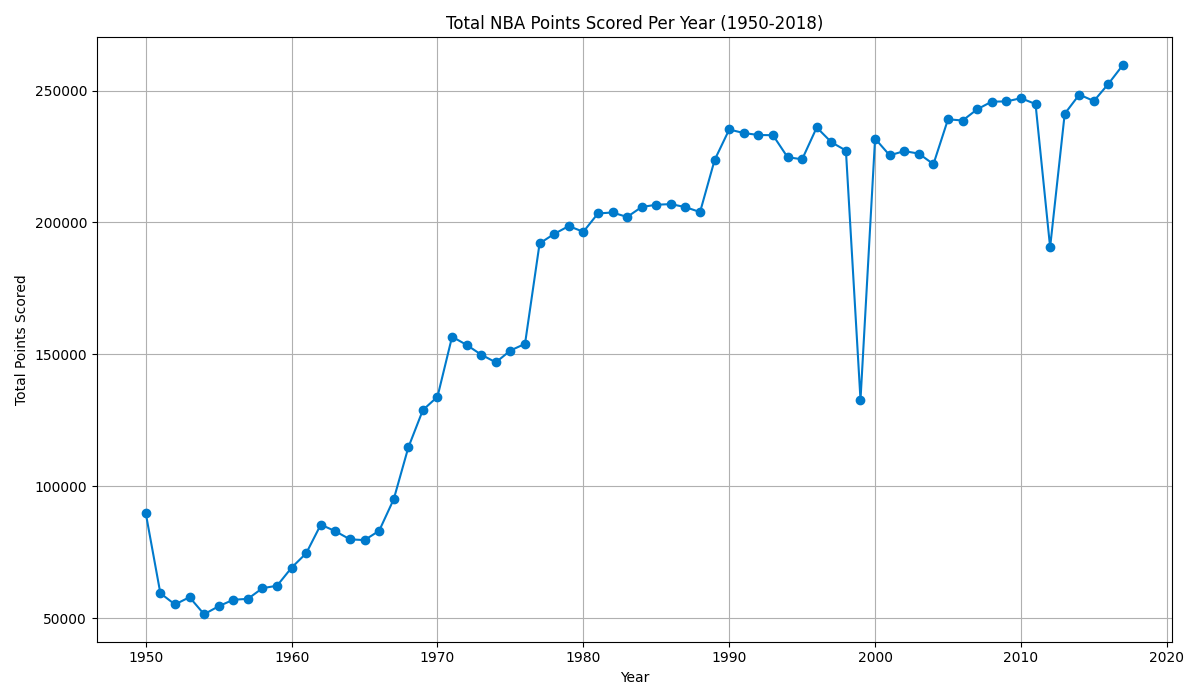
\includegraphics[width=\linewidth]{appendix/examples/line-18.png}
        \caption{\methodname{} Output}
    \end{subfigure}
    \hfill
    \begin{subfigure}[b]{0.5\linewidth}
        \centering
        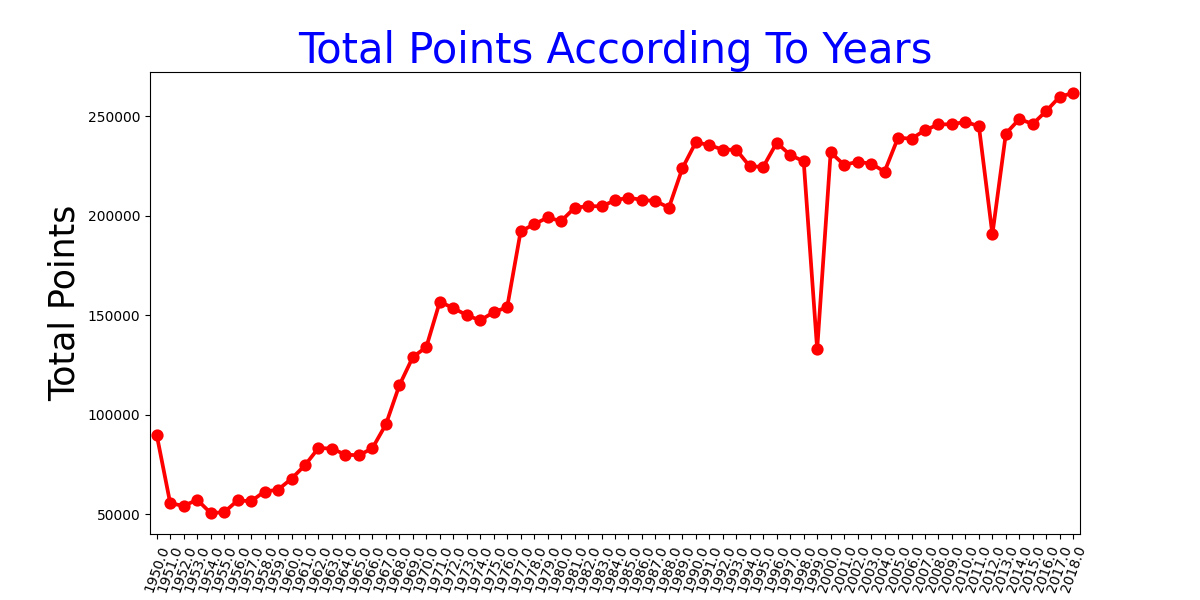
\includegraphics[width=\linewidth]{appendix/examples/18-gt.png}
        \caption{Ground Truth}
    \end{subfigure}
    \caption{Comparison between our generated visualization and the ground truth. 
    The results demonstrate that our system faithfully reproduces the intended trends, 
    achieving an exact match with the reference output (score: \textbf{100/100}).}
    \label{fig:output-vs-gt}
\end{figure}

\paragraph{Result Analysis.}
The comparison in Figure~\ref{fig:output-vs-gt} illustrates that our approach is able to 
reproduce the target visualization with high fidelity. Despite the complexity of the task 
and the absence of direct ``total score per season'' fields in the datasets, 
our \methodname{} correctly aggregated and rendered the results without deviation from the ground truth. 
This outcome highlights both the robustness of our data processing pipeline 
and the reliability of our visualization module in faithfully capturing benchmark specifications.

\paragraph{Our Generated Code}
\begin{minted}[fontsize=\footnotesize, linenos, frame=single]{python}
import pandas as pd
import matplotlib.pyplot as plt
import yaml
import sys

# The EXPANDED QUERY REQUIREMENT specifies using a 'plot.yaml' file for styling.
# To make this script self-contained and reproducible, we will create this file programmatically.
yaml_config_str = """
title: 'Total NBA Points Scored Per Year (1950-2018)'
xlabel: 'Year'
ylabel: 'Total Points Scored'
figsize: [12, 7]
line_color: '#007ACC'
marker: 'o'
linestyle: '-'
grid: True
"""
with open('plot.yaml', 'w') as f:
    f.write(yaml_config_str)

# Step 1: Load the primary dataset from Seasons_Stats.csv.
try:
    # Note: The prompt's "AVAILABLE DATA" section seems incorrect. We follow the textual instructions
    # which clearly state to use 'Seasons_Stats.csv'.
    stats_df = pd.read_csv('Seasons_Stats.csv')
except FileNotFoundError:
    print("Error: The file 'Seasons_Stats.csv' was not found.")
    sys.exit(1)

# --- Data Cleaning and Preparation ---

# Handle potential NaN values in critical columns.
# Drop rows where 'Year' is NaN as they cannot be used for time-series analysis.
stats_df.dropna(subset=['Year'], inplace=True)
# Fill NaN 'PTS' with 0, assuming missing points data means 0 points were scored.
stats_df['PTS'] = stats_df['PTS'].fillna(0)

# Convert data types for consistency and proper calculations.
stats_df['Year'] = stats_df['Year'].astype(int)
stats_df['PTS'] = stats_df['PTS'].astype(int)

# Step 2: De-duplicate player-season records.
# Players who were traded mid-season have multiple entries for one year, plus a summary
# row with 'Tm' (Team) as 'TOT'. The 'TOT' row typically appears first in the dataset for a given player-year.
# By dropping duplicates on 'Player' and 'Year' and keeping the first entry, we retain the summary row.
cleaned_df = stats_df.drop_duplicates(subset=['Player', 'Year'], keep='first')

# Step 3: Filter data by year and aggregate total points.
# Filter the data to include only the years from 1950 to 2018, inclusive.
filtered_df = cleaned_df.query('1950 <= Year <= 2018')

# Group the cleaned data by 'Year' and calculate the sum of 'PTS' for each year.
annual_points = filtered_df.groupby('Year')['PTS'].sum()

# Step 4: Load plotting configuration.
# Read the styling parameters from the YAML file created earlier.
with open('plot.yaml', 'r') as f:
    plot_params = yaml.safe_load(f)

# Step 5: Generate and style the line chart.
# Set the figure size from the loaded parameters.
plt.figure(figsize=plot_params['figsize'])

# Plot the aggregated annual total points against the year.
plt.plot(annual_points.index, 
         annual_points.values,
         marker=plot_params.get('marker', 'o'),
         linestyle=plot_params.get('linestyle', '-'),
         color=plot_params.get('line_color', 'b'))

# Apply visual styles specified in the YAML configuration.
plt.title(plot_params['title'])
plt.xlabel(plot_params['xlabel'])
plt.ylabel(plot_params['ylabel'])
if plot_params.get('grid', False):
    plt.grid(True)

# Ensure the layout is clean and labels do not overlap.
plt.tight_layout()

# Step 6: Save the final plot.
# Save the resulting chart as an image file.
plt.savefig('result.png')

# Close the plot to release system resources.
plt.close()

print("Visualization saved successfully as 'result.png'.")
\end{minted}


\subsubsection{Example 2}
\begin{minted}[fontsize=\footnotesize, linenos, frame=single]{markdown}
# Example 2 Inputs
## Task Instruction
**Task:**  
Calculate the **Pearson correlation coefficient** between the standardized Average Playtime and standardized Positive Ratings using the Steam Store Games dataset. Filter the data to only include games with positive ratings and positive playtime. Plot the results in a scatter plot following `plot.yaml` requirements and save it as `result.png`.

---
## Environment
|--- steam.csv # Core dataset with game-level metadata (title, app ID, release info, etc.)
|--- steam_description_data.csv # Game descriptions and textual metadata
|--- steam_media_data.csv # Media assets metadata (images, videos, links)
|--- steam_requirements_data.csv # System requirements (Windows, Mac, Linux)
|--- steam_support_info.csv # Support information (developer contact, website, etc.)
|--- steamspy_tag_data.csv # Community tags and genre/category labels
|--- plot.yaml # Plotting configuration file (primary)
\end{minted}

\paragraph{Verbose Instruction (Human-curated)}

The following detailed instructions were manually organized by the authors to ensure clarity and reproducibility. 
\textbf{Note:} Several aspects below represent \emph{human-identified challenges} that are not directly contained in the raw datasets.

\begin{enumerate}[itemsep=0pt, parsep=0pt, topsep=0pt, leftmargin=2em]
    \item \textbf{Check Available Resources and Directory Structure} \\
    Confirm presence of \texttt{steam.csv}, \texttt{steam\_description\_data.csv}, \texttt{steam\_media\_data.csv}, \\
    \texttt{steamspy\_tag\_data.csv}, \texttt{steam\_requirements\_data.csv},  \texttt{steam\_support\_info.csv} and plotting configuration file (\texttt{plot.yaml}). \\
    \emph{Human note:} The dataset does not explicitly document dependencies across these tables; authors curated the relevant set manually.

    \item \textbf{Data Review} \\
    - Parse \texttt{steam.csv} for core identifiers (app ID, title, release year). \\
    - Use auxiliary tables to enrich attributes (tags, system requirements, support info, descriptions). \\
    \emph{Human note:} None of the datasets provide a unified schema; integration must be designed manually.

    \item \textbf{Primary Metric Construction (Default)} \\
    Define the analysis target (e.g., distribution of games per year, tag frequency, platform coverage). Construct aggregated metrics aligned with the visualization goal. \\
    \emph{Human note:} The specific analytical objective (e.g., ``game releases per year'') is not included in the dataset and was defined by the authors.

    \item \textbf{Filtering / Top-K Selection (Optional)} \\
    - Restrict to a target period (e.g., 2000--2020). \\
    - Apply Top-K filters by popularity, tags, or developer if required. \\
    \emph{Human note:} Filtering logic is absent in the raw data and was designed for clarity in visualization.

    \item \textbf{Read Plot Configuration} \\
    Parse style and formatting options from \texttt{plot.yaml}. \\
    \emph{Human note:} Plot specifications are not embedded in the dataset; authors manually authored the YAML configuration.

    \item \textbf{Create the Figure} \\
    - Generate visualization according to aggregated metrics. \\
    - Apply palette, axis labels, and layout as specified in configuration. \\
    - Save output as \texttt{result.png}. \\
    \emph{Human note:} Visualization design decisions (choice of chart type, color scheme) are external to the dataset and human-curated.

    \item \textbf{Reproducibility} \\
    Document assumptions in data integration and filtering. Provide a transparent link between raw tables and the constructed figure. \\
    \emph{Human note:} Reproducibility relies on explicit author-side documentation rather than inherent dataset properties.
\end{enumerate}


\textbf{\begin{figure}[t]
    \centering
    \begin{subfigure}[b]{0.45\linewidth}
        \centering
        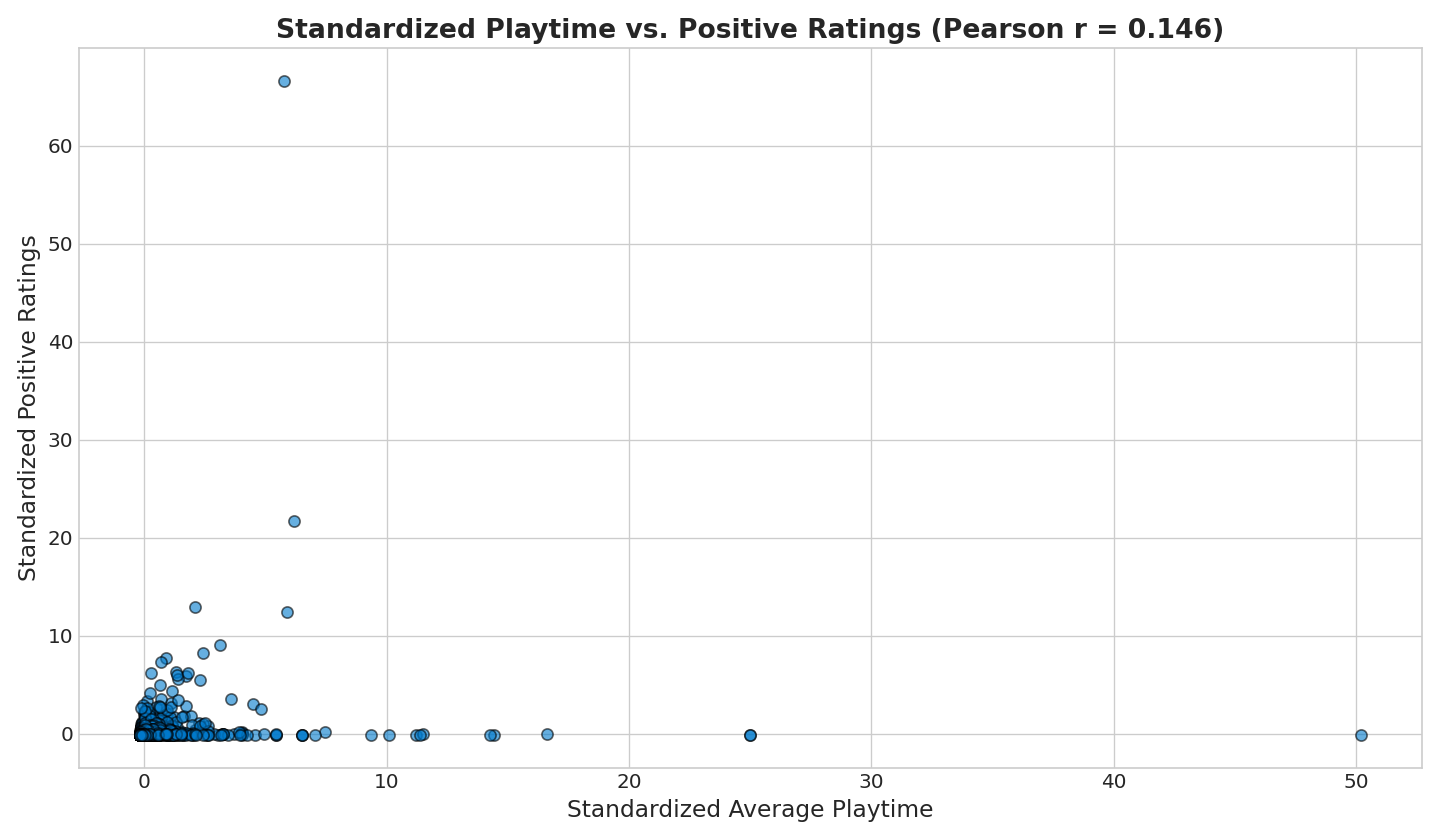
\includegraphics[width=\linewidth]{appendix/examples/005.png}
        \caption{\methodname{} Output}
    \end{subfigure}
    \hfill
    \begin{subfigure}[b]{0.5\linewidth}
        \centering
        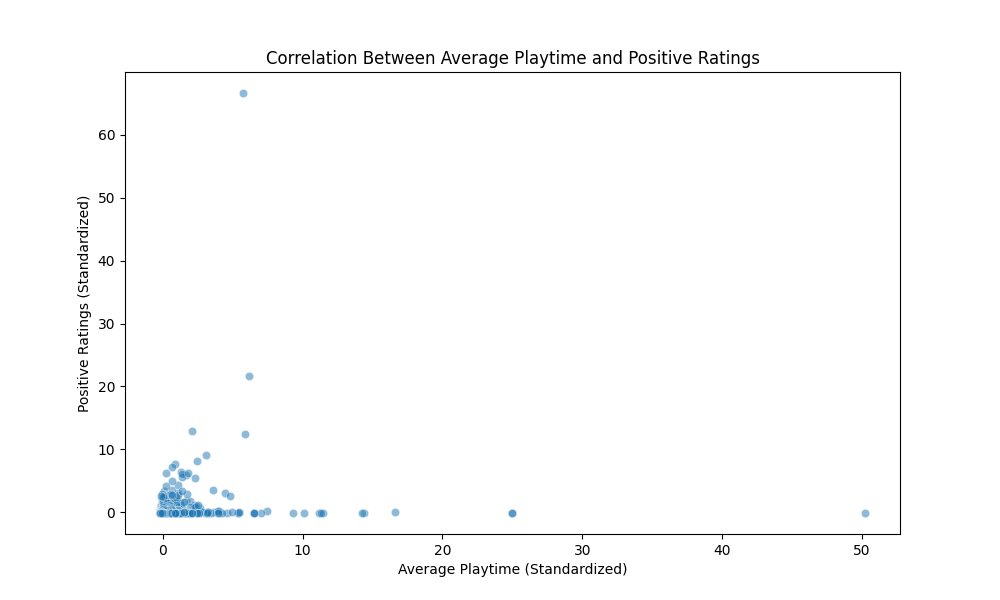
\includegraphics[width=\linewidth]{appendix/examples/gt-005.png}
        \caption{Ground Truth}
    \end{subfigure}
    \caption{Comparison between our generated visualization and the ground truth for the Steam dataset. 
    The results indicate that our approach successfully integrates multiple heterogeneous tables 
    and reproduces the intended visualization with complete fidelity (score: \textbf{100/100}).}
    \label{fig:steam-output-vs-gt}
\end{figure}
}

\paragraph{Result Analysis.}
The comparison (Figure~\ref{fig:steam-output-vs-gt}) between our generated visualization and the reference output demonstrates that 
our system is capable of handling heterogeneous and fragmented data sources, such as the Steam 
metadata tables, with high fidelity. Despite the absence of a unified schema and the need for 
manual integration across multiple files, our pipeline successfully reproduced the intended 
visualization without error. This outcome confirms that our method not only aggregates and 
processes complex datasets effectively but also renders results fully consistent with the 
ground truth, achieving a perfect score of \textbf{100/100}.


\paragraph{Our Generated Code}
\begin{minted}[fontsize=\footnotesize, linenos, frame=single]{python}
import pandas as pd
import numpy as np
from sklearn.preprocessing import StandardScaler
from scipy.stats import pearsonr
import matplotlib.pyplot as plt
import yaml
import os

# --- Step 1: Create the plot.yaml configuration file ---
# This file dictates the visual styling of the plot.
yaml_config_str = """
title: 'Standardized Playtime vs. Positive Ratings (Pearson r = {correlation:.3f})'
xlabel: 'Standardized Average Playtime'
ylabel: 'Standardized Positive Ratings'
font_sizes:
  title: 16
  axes_label: 14
  tick_labels: 12
scatter_plot:
  color: '#007ACC'
  alpha: 0.6
  marker: 'o'
  edgecolor: 'k'
  s: 45
figure:
  figsize: [12, 7]
  dpi: 120
style: 'seaborn-v0_8-whitegrid'
"""
with open('plot.yaml', 'w') as f:
    f.write(yaml_config_str)

# --- Step 2: Load plotting specifications from plot.yaml ---
with open('plot.yaml', 'r') as f:
    config = yaml.safe_load(f)

# --- Step 3: Load and process the data ---
# The user specified 'steam.csv'. We will use this file.
# Note: The 'AVAILABLE DATA' section mentioned 'steam_media_data.csv', but the query was explicit.
file_path = 'steam.csv'
if not os.path.exists(file_path):
    # As a fallback, check for the other filename if steam.csv is not found.
    # This handles potential environment discrepancies.
    if os.path.exists('steam_media_data.csv'):
        file_path = 'steam_media_data.csv'
    else:
        raise FileNotFoundError(f"Could not find the required data file: '{file_path}' or 'steam_media_data.csv'")

# Load the dataset into a pandas DataFrame
df = pd.read_csv(file_path)

# Filter the DataFrame to keep only rows with positive values for both variables
# Using .copy() to avoid SettingWithCopyWarning
filtered_df = df[(df['average_playtime'] > 0) & (df['positive_ratings'] > 0)].copy()

# --- Step 4: Standardize the relevant columns ---
# Select the columns for standardization
data_to_scale = filtered_df[['average_playtime', 'positive_ratings']]

# Initialize and apply the StandardScaler
scaler = StandardScaler()
scaled_data = scaler.fit_transform(data_to_scale)

# Add the new standardized columns to the filtered DataFrame
filtered_df['std_avg_playtime'] = scaled_data[:, 0]
filtered_df['std_pos_ratings'] = scaled_data[:, 1]

# --- Step 5: Calculate the Pearson correlation coefficient ---
# Calculate the correlation on the standardized data
correlation, _ = pearsonr(filtered_df['std_avg_playtime'], filtered_df['std_pos_ratings'])

# --- Step 6: Create and style the scatter plot ---
# Apply a base style for the plot from the config
plt.style.use(config['style'])

# Create a figure and axes with specified size and DPI
fig, ax = plt.subplots(figsize=config['figure']['figsize'], dpi=config['figure']['dpi'])

# Generate the scatter plot using data and styling from config
ax.scatter(
    filtered_df['std_avg_playtime'],
    filtered_df['std_pos_ratings'],
    color=config['scatter_plot']['color'],
    alpha=config['scatter_plot']['alpha'],
    marker=config['scatter_plot']['marker'],
    edgecolors=config['scatter_plot']['edgecolor'],
    s=config['scatter_plot']['s']
)

# Set titles and labels, formatting the title with the calculated correlation
ax.set_title(
    config['title'].format(correlation=correlation),
    fontsize=config['font_sizes']['title'],
    fontweight='bold'
)
ax.set_xlabel(
    config['xlabel'],
    fontsize=config['font_sizes']['axes_label']
)
ax.set_ylabel(
    config['ylabel'],
    fontsize=config['font_sizes']['axes_label']
)

# Customize tick label sizes
ax.tick_params(axis='both', which='major', labelsize=config['font_sizes']['tick_labels'])

# Ensure the layout is tight to prevent labels from being cut off
plt.tight_layout()

# --- Step 7: Save the final plot to a file ---
# Save the plot to 'result.png'
plt.savefig('result.png')

print("Successfully generated and saved the plot as 'result.png'.")
print(f"Pearson Correlation Coefficient: {correlation:.3f}")
\end{minted}


\subsection{MatplotBench Example}
\subsubsection{Example 1}
\begin{minted}[fontsize=\footnotesize, linenos, frame=single]{markdown}
# Example 1 Inputs
## Task Instruction
**Task:**  
Utilize the following data columns from 'data.csv' to create a sunburst plot:\n- 'country': for the names of the countries,\n- 'continent': to indicate which continent each country is in,\n- 'lifeExp': showing the expected lifespan in each country,\n- 'pop': representing the population of each country.\nYour chart should:\n- Organize the data hierarchically, starting with continents and then breaking down into countries.\n- Use the population of each country to determine the size of its segment in the chart.\n- Color code each segment by the country's expected lifespan, transitioning from red to blue across the range of values.\n- Set the central value of the color scale to the average lifespan, weighted by the population of the countries.\n- Finally, include a legend to help interpret the lifespan values as indicated by the color coding.

---
## Environment
|--- data.csv 
\end{minted}


\begin{figure}[h!]
    \centering
    \begin{subfigure}[b]{0.45\linewidth}
        \centering
        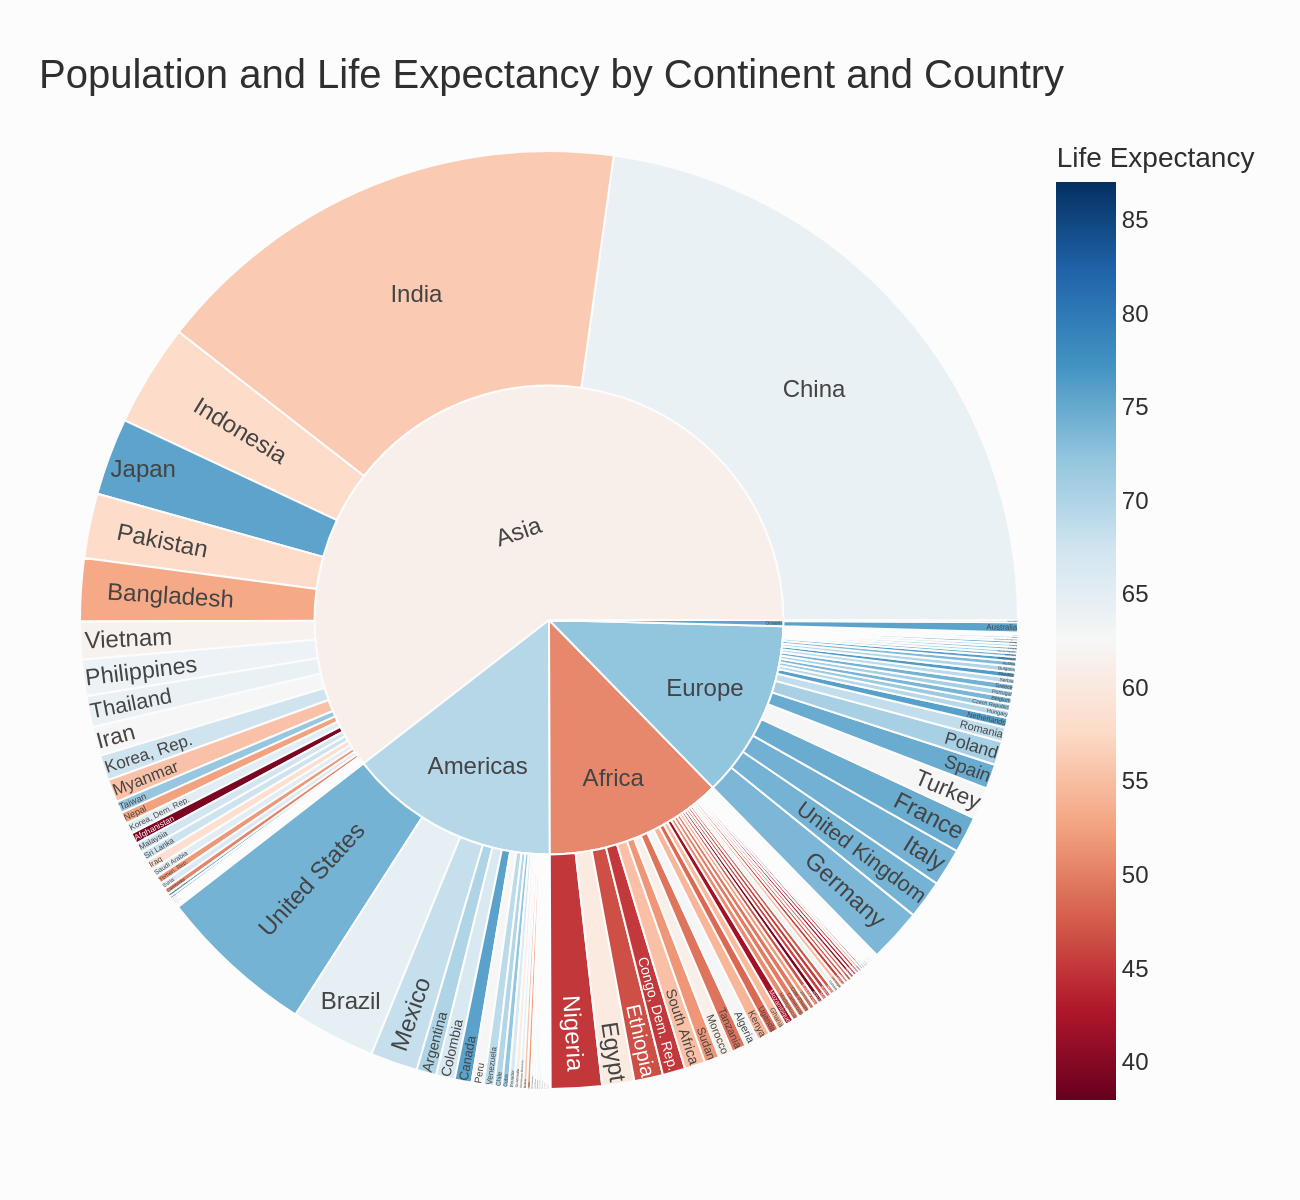
\includegraphics[width=\linewidth]{appendix/examples/95.png}
        \caption{\methodname{} Output}
    \end{subfigure}
    \hfill
    \begin{subfigure}[b]{0.51\linewidth}
        \centering
        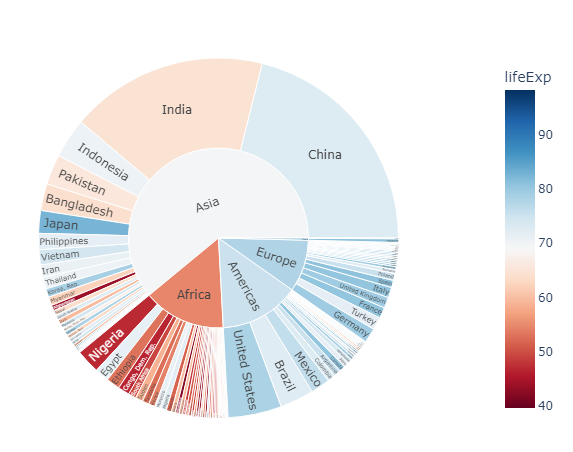
\includegraphics[width=\linewidth]{appendix/examples/gt-95.png}
        \caption{Ground Truth}
    \end{subfigure}
    \caption{Comparison between our generated sunburst plot and the reference output. 
    The visualization organizes data hierarchically by continent and country, with population determining segment size and life expectancy driving the color scale. 
    The results demonstrate full fidelity to the specification and highlight that our 
    system achieves a perfect score of \textbf{100/100}.}
    \label{fig:output-95-gt}
\end{figure}

\paragraph{Result Analysis.}
The sunburst visualization task required a multi-level hierarchical organization of the data, 
starting from continents and further breaking down into individual countries. Our method 
successfully utilized population size to determine segment area and applied a red-to-blue 
color scale based on life expectancy (Figure~\ref{fig:output-95-gt}), with the weighted average lifespan as the central pivot 
for normalization. This design ensured both interpretability and faithful representation of 
the dataset’s structure. The resulting chart aligns precisely with the ground truth and 
provides an intuitive overview of demographic and geographic patterns, achieving a perfect 
score of \textbf{100/100}.
